\section{Long-Only Q1 Cumulative Returns}
\label{app:q1-cumret}

Figure~\ref{fig:q1-cumret} shows the cumulative wealth path of the top-quintile (Q1) long-only portfolio for each model and prediction mode.
These trajectories combine the ranking signal with broad market exposure and are therefore more sensitive to market direction than the Q1$-$Q5 spread in the main text; the equal-weighted universe line helps separate stock-selection gains from the common AI-rally market drift.

\begin{figure}[H]
  \centering
  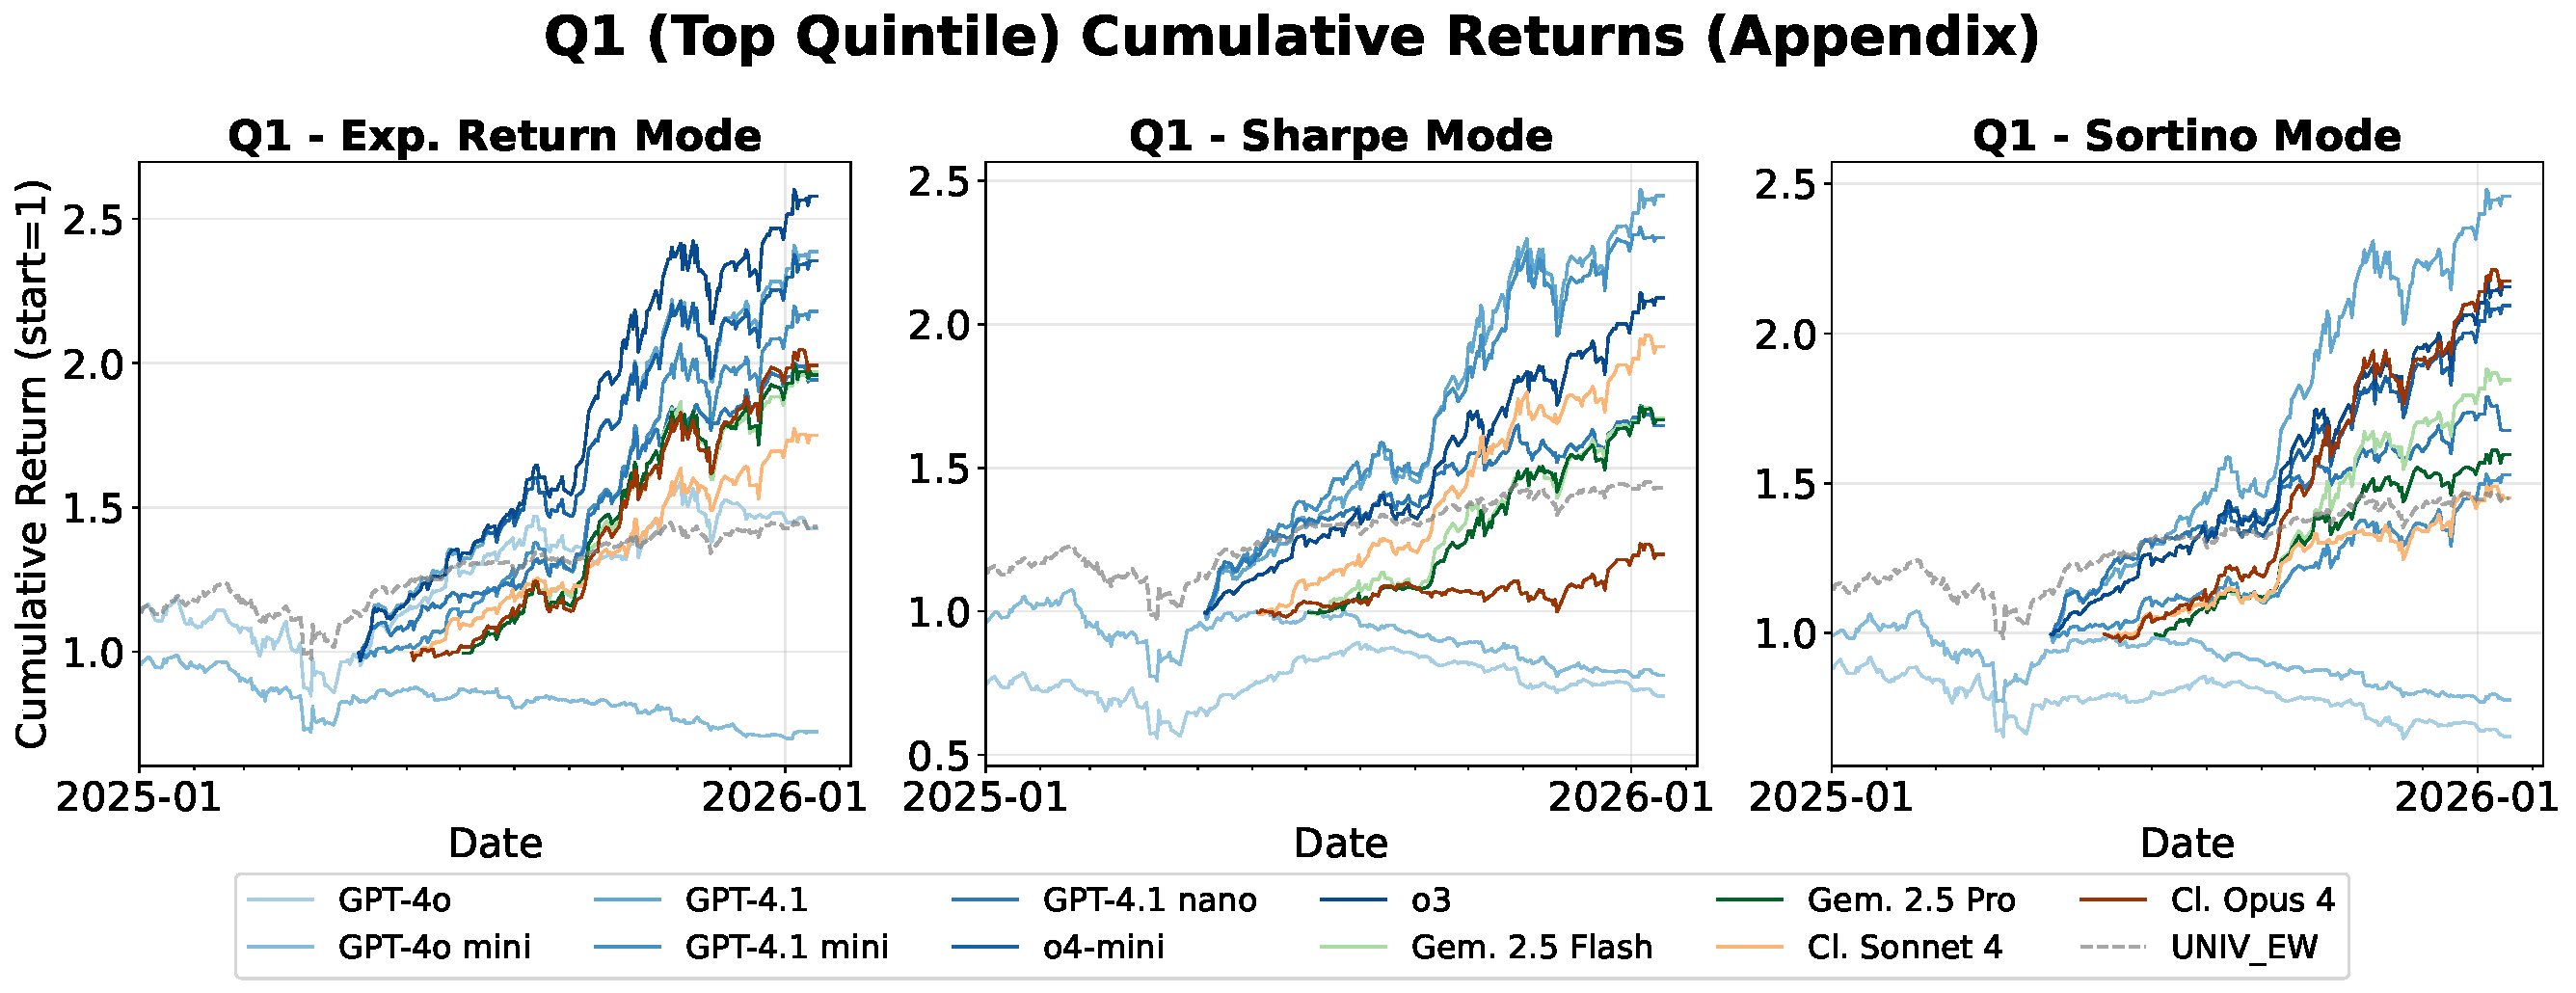
\includegraphics[width=\textwidth]{figures/fig6_q1_cumulative_returns.pdf}
  \caption{Cumulative wealth of Q1 long-only portfolios by model and prediction mode. The dashed gray line is the equal-weighted universe benchmark.}
  \Description{Line plots of cumulative top-quintile long-only wealth for each model and prompt objective, with a benchmark line for the equal-weighted universe and different path start dates reflecting conservative windows.}
  \label{fig:q1-cumret}
\end{figure}

The Q1 paths reinforce why the main text emphasizes Q1$-$Q5 spreads rather than long-only returns alone.
Several strong models participate in the broad AI-market rally, but the market-neutral spread tests whether the same ranking also avoids the weak bottom quintile.
Thus, Figure~\ref{fig:q1-cumret} is best read as a long-only decomposition of the stronger cross-sectional evidence in Table~\ref{tab:longshort}.

% ──────────────────────────────────────────────────────────────
\clearpage
